\chapter{Algoritmo de Navegaci\'on aut\'onoma}\label{cap.algoritmo} %Algoritmo de Navegaci\'on aut\'onoma

\hspace{1 cm} En este cap\'itulo se describe el modo por el cual, con la infraestructura que se tiene, se ha llegado a una soluci\'on para los objetivos planteados. 

\hspace{1 cm} Este algoritmo tiene que permitir al drone despegar de forma controlada, realizar una navegaci\'on aut\'onoma para encontrar una baliza sobre la que aterrizar. La organizaci\'on de este cap\'itulo tiene primero una secci\'on de diseño en la que se explica el funcionamiento del programa. Tras esto una secci\'on de percepci\'on para explicar los datos que se obtienen a trav\'es de los sensores. Una secci\'on de control, para explicar los distintos movimientos del drone y de que dependen estos. Y finalmente se explica la arquitectura software en la que se han programado las partes perceptivas y de control del algoritmo.

\section{Diseño}
\label{sec.Design}

\hspace{1 cm} El diseño de este algoritmo consta de un comportamiento reactivo de iteraciones continuas. Es un proceso basado en adquisici\'on-procesado-env\'io de ordenes, tal y como muestra la figura \ref{fig:esquema_d1}. La adquisici\'on de los datos se realizan mediante los sensores del drone. Estos datos sensoriales ser\'an recogidos para su procesamiento y tras \'esto se enviar\'an las instrucciones al drone para que las ejecute. El sensor utilizado en este proyecto ha sido la c\'amara, y los movimientos del drone depender\'an de lo que esta capte en cada momento. 

\hspace{1 cm} Por otro lado, la parte de control es un aut\'omata finito de estados, el cual comienza en un estado inicial (despegue), y en funci\'on de lo que recibe a la entrada (imagen del sensor), realizar\'a el procesamiento necesario para producir la informaci\'on que enviar al drone, y en ocasiones le llevar\'a a pasar de un estado a otro. Este aut\'omata est\'a compuesto por 6 estados: despegando, buscando, posible baliza, centr\'andose en la baliza, aterrizando y aterrizado. A excepci\'on del primero, los dem\'as estados depender\'an de lo que detecte el drone en cada momento. El primer estado est\'a controlado por tiempo, pues son 10 segundos al iniciarse en los que el drone inicia el vuelo sobre una baliza y trata de estar centrado sobre \'esta, para as\'i tener un despegue controlado y evitar que el drone se mueva en caso de tener alguna deriva o haya factores externos que produzcan esto. Una vez transcurridos los 10 segundos se pasar\'a al estado de b\'usqueda e ir\'a pasando por los distintos estados hasta su aterrizaje, seg\'un se explicar\'a con detalle en la secci\'on \ref{sec.control}. 

\begin{figure}[H]
	\centering
		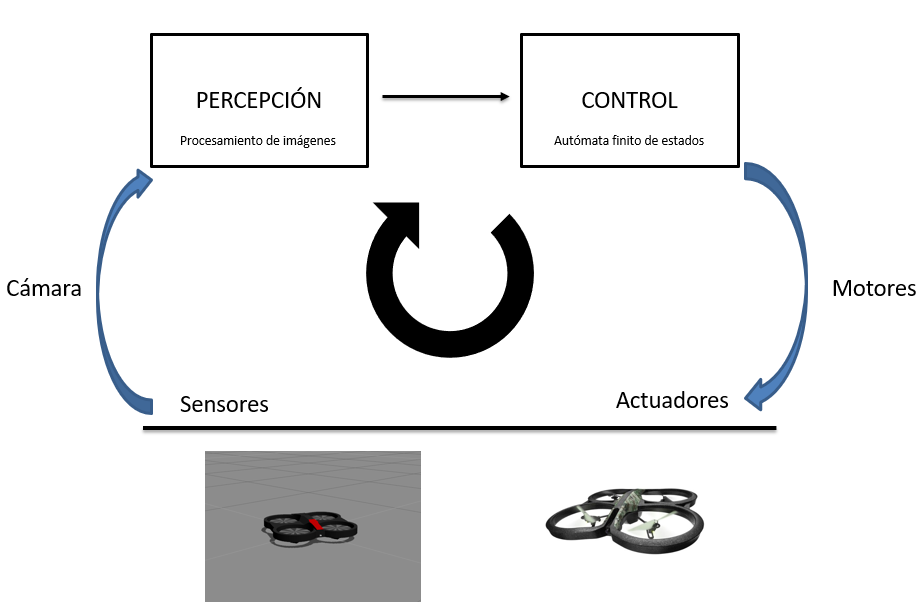
\includegraphics[width=0.75\textwidth]{imgs/esquema2.png}
         \caption{Esquema que muestra la adquisici\'on, proceso y envio de ordenes}
	\label{fig:esquema_d1}
\end{figure}

\hspace{1 cm} El lugar de aterrizaje del drone es una baliza previamente definida \ref{fig:esquema_d}. Esta baliza es un cuadrado que en su interior tiene cuatro cuadrantes, dos naranjas, y dos azules o verdes, dependiendo si se trabaja con el drone real o con el simulador. Esta baliza se diseñ\'o as\'i para que sea dif\'icil confundirla con otro objeto, pues de ser una baliza simple se podr\'ian confundir los colores y para que se pudiera detectar del mismo modo a diferentes alturas. Lo que busca el software ser\'a la cruceta que forman estos cuatro cuadrados y el punto central de \'esta. Lo que buscar\'a es un objeto que tenga determinadas caracter\'isticas y patrones, algo que se puede detectar a diferentes alturas, distintas condiciones y situaciones.

\begin{figure}[H]
	\centering
		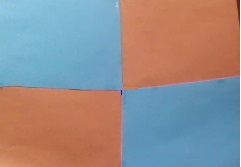
\includegraphics[width=0.2\textwidth]{imgs/baliza.jpg}
         \caption{Baliza utilizada para el drone real.}
	\label{fig:esquema_d}
\end{figure}


\hspace{1 cm} Por \'ultimo, para el control del drone con nuestro algoritmo se ha utilizado la herramienta \textit{follow\_turtlebot} de JdeRobot Academy, explicada en \ref{sec.JdeRobotAcademyFT}. Esta aplicaci\'on tiene un interfaz gr\'afico de usuario (GUI) que permite controlar el drone y ver los datos de los distintos sensores, as\'i como la imagen que obtiene la c\'amara. Por otro lado, cuenta con las interfaces ICE que permite la comunicaci\'on con el servidor, pudiendo as\'i recibir datos de sensores y motores, y enviar las instrucciones de velocidad necesarias en cada momento. La imagen de la aplicaci\'on se encuentra en la figura \ref{fig:FollowTurtlebot}


\section{Percepci\'on}

\hspace{1 cm} En esta secci\'on se va a tratar la obtenci\'on de la imagen de la c\'amara y el procesamiento que se realiza sobre \'esta. Gracias a lo que el drone ve en todo momento, sabe el punto del comportamiento en el que se encuentra y la informaci\'on que debe enviar. En primer lugar se obtiene una imagen de entrada. Esta imagen es procesada con filtros de color y operadores morfol\'ogicos, obteniendo una imagen de salida. A partir de los datos de esta imagen, se detecta si hay objetos de inter\'es o no, y por tanto se env\'ia unas instrucciones u otras al drone. 


\begin{figure}[H]
	\centering
		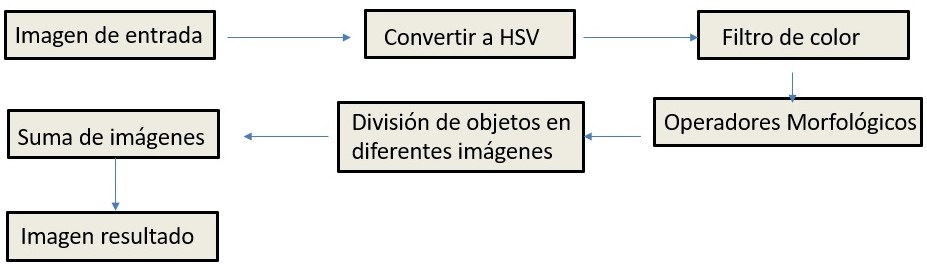
\includegraphics[width=1\textwidth]{imgs/fig421.jpg}
        \caption{Esquema de percepcion del algoritmo}
	\label{fig:Procesado_percepcion}
\end{figure}

\subsection{Pre-procesado}

\hspace{1 cm} Una vez tenemos la imagen de entrada, hay que detectar la informaci\'on de inter\'es que nos aporta.  En primer lugar, la imagen que est\'a en RGB se transforma a HSV, para que sea m\'as facil su interpretaci\'on, ya que en lugar de trabajar en funci\'on de tres colores puros (rojo, verde y azul) se trabaja en funci\'on de tres par\'ametros (tono, saturaci\'on y valor). De esta forma, se depende menos de la luz que haya en cada momento y en cada lugar.En segundo lugar se pasan los filtros de color a la imagen. En el filtro a cada uno de los par\'ametros se le asigna un rango de valores entre 0 y 255. La herramienta \textit{colorTuner} de JdeRobot permite, a partir de una imagen de entrada, dar valores a estos par\'ametros, viendo que objetos cumplen estos requisitos y dej\'andolos en primer plano, y cuales no, dejando estas zonas en negro como p\'ixeles de fondo. Una vez se obtienen estos valores se añaden al filtro, obteniendo a la salida una imagen que solo muestra los objetos de los colores de inter\'es. 

\hspace{1 cm} El siguiente c\'odigo es un ejemplo de como a partir de una imagen de entrada en RGB, se transforma a HSV y se filtran los objetos de color naranja. 

\begin{lstlisting}[backgroundcolor=\color{yellow}]
hsv = cv2.cvtColor(input_image, cv2.COLOR_BGR2HSV)
lower_orange = np.array([100,100,80], dtype=np.uint8)
upper_orange = np.array([150, 255,255], dtype=np.uint8)
maskOrange = cv2.inRange(hsv, lower_orange, upper_orange)
maskRGBOrange = cv2.bitwise_and(input_image,input_image, mask= maskOrange)
\end{lstlisting}


\hspace{1 cm} En caso de trabajar sobre simulador, con esto se obtiene a la salida una imagen bastante parecida a la deseada, debido a la pureza de los colores. Sin embargo, al trabajar sobre im\'agenes reales, la imagen de salida de este filtro a\'un tiene ruido y objetos de inter\'es imperfectos. Para arreglar esto se utilizan los operadores morfol\'ogicos, que eliminan estas imperfecciones. Una breve explicaci\'on de los utilizados es la siguiente: 

\begin{itemize}
	\item \textbf{Erosi\'on:} Operaci\'on morfol\'ogica que comprime los p\'ixeles en primer plano, eliminando asi p\'ixeles aislados.
	\item \textbf{Dilataci\'on:} Transformaci\'on dual a la erosi\'on. Operaci\'on morfol\'ogica que dilata los p\'ixeles en primer plano.
	\item \textbf{Cierre:} Realizar una dilataci\'on en la imagen seguida de una erosi\'on.
	\item \textbf{Apertura:} Realizar la erosi\'on en una imagen seguida de una dilataci\'on.
\end{itemize}


\hspace{1 cm} De esta forma, al obtener una imagen sin apenas ruido, se evita que objetos de no inter\'es los detecte como tal y que los objetos de inter\'es los trate como p\'ixeles de fondo.La figura \ref{fig:E_Imagen_baliza} muestra la realizaci\'on de un filtro de color y el uso de operadores morfol\'ogicos:

\begin{figure}[ht]
	\centering
		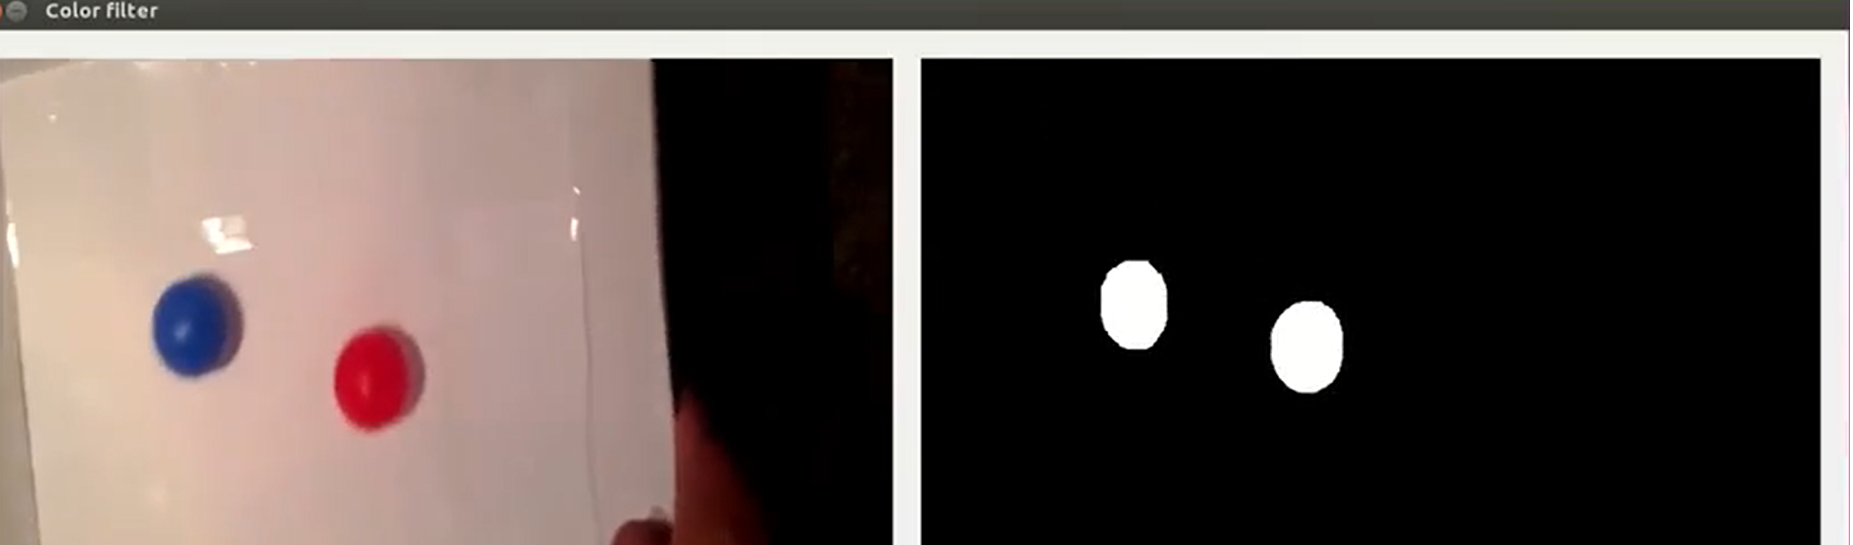
\includegraphics[width=0.8\textwidth]{imgs/colorfilter.eps}
         \caption{Ejemplo de un filtro de color y uso de operadores morfol\'ogicos para eliminar ruido.}
	\label{fig:E_Imagen_baliza}
\end{figure}


\hspace{1 cm} El siguiente fragmento de c\'odigo muestra c\'omo se define la matriz a partir de la cual se realizar\'an las operaciones oportunas y se realizan la erosi\'on y la dilataci\'on.
\begin{lstlisting}[backgroundcolor=\color{yellow}]
kernel = np.ones((3,3),np.uint8)
maskRGBOrange = cv2.erode(maskRGBOrange,kernel,iterations = 4)
maskRGBOrange = cv2.dilate(maskRGBOrange,kernel,iterations = 3)
\end{lstlisting}


\subsection{Detecci\'on de la baliza}
\hspace{1 cm} Una vez se obtienen los colores de los objetos de inter\'es, hay que buscar el objeto deseado. Para esto hay que buscar el punto de intersecci\'on entre los cuatro cuadrados de la baliza. Para ello los pasos a realizar son los siguientes:

\begin{enumerate}
	\item Para la imagen de entrada se hacen dos filtros de color, uno por cada color de la baliza tal y como se ha descrito en la subsecci\'on previa.
	\item De cada imagen se obtienen el n\'umero de objetos, las \'areas y los contornos. En cada objeto se obtiene el valor de su \'area, en caso de ser menor de un valor determinado, se descarta. En caso de tener ese \'area o mayor, se crea una imagen negra, se pintan los contornos del objeto sobre \'esta con un valor RGB(0,1,0) y se dilatan. De esta forma, tendremos tantas im\'agenes como objetos. 
	\item Se suman las im\'agenes obtenidas. Sobre una imagen negra final se pintan los contornos dilatados de todos los objetos. Cada contorno se pintar\'a con un valor RGB(0,1,0), por lo tanto en el caso de que varios objetos coincidan sumar\'an sus valores. Con esto conseguiremos que el punto donde interseccionen cuatro objetos tenga un valor (0,4,0), y por tanto ser\'a el centro de la cruceta.
	
\hspace{1 cm}El siguiente fragmento de c\'odigo muestra la creaci\'on de una imagen por objeto, la dilataci\'on de los contornos y la suma final de las im\'agenes:

\begin{lstlisting}[backgroundcolor=\color{yellow}]
f = []
i=0
imgray2 = cv2.cvtColor(maskRGBOrange,cv2.COLOR_BGR2GRAY)
ret,thresh = cv2.threshold(imgray2,255,255,255)
_,contours, hierarchy = cv2.findContours(thresh,cv2.RETR_TREE,
                                          cv2.CHAIN_APPROX_SIMPLE)
\'areas = [cv2.contour\'area(c) for c in contours]
for extension in \'areas:
    if extension > 100:
    img = np.zeros((y_img*2,x_img*2,3), np.uint8)
        actual = contours[i]
        approx = cv2.approxPolyDP(actual,0.05*cv2.arcLength(actual,True),
                                                                       True)
        cv2.drawContours(img,[actual],0,(0,30,0),12)
        f.append(img)
        i=i+1
			
kernel = np.ones((3,3),np.uint8)
if(len(f)>0):
    f[0] = cv2.dilate(f[0],kernel,iterations = 4)
    show_image2=f[0]
    for k in range(len(f)-1):
        f[k+1] = cv2.dilate(f[k+1],kernel,iterations = 4)
        show_image2=show_image2+f[k+1]
		
\end{lstlisting}


	\item A partir de la imagen final, se pasar\'a un filtro que se quedar\'a solo con los valores mayores a RGB(0,3,0), por lo tanto el \'unico valor que no se eliminar\'a sera el del centro de la cruceta.

	\item Sobre la imagen obtenida, utilizando la funci\'on \textit{drawcontours}, se obtienen la situaci\'on de las fronteras entre cuadrantes y de la cruceta, y con estos valores se puede marcar el centro de la baliza sobre la imagen real. Para visualizar en el GUI, se puede hacer que el filtro deje pasar valores mayores o iguales a RGB(0,2,0) obteniendo as\'i las fronteras entro los cuadrantes, o los valores mayores o igual a RGB(0,1,0), obteniendo asi los cuadrantes de los objetos. Al dejar pasar m\'as objetos en el filtro y por tanto no ser tan robusto, puede tener en ocasiones falsos positivos.

\hspace{1 cm}En el siguiente fragmento de c\'odigo se muestra como a partir de la imagen de la suma de objetos, se calcula la posici\'on de la cruceta y se marcan sobre la imagen. En este caso, para que se obtuviera una imagen m\'as clara, a los bordes de los objetos se les da un valor de 30, por lo tanto la intersecci\'on de 3 objetos tendr\'a un valor RGB(0,90,0) y de 4 objetos un valor RGB(0,120,0).

\begin{lstlisting}[backgroundcolor=\color{yellow}]
lower_green = np.array([0,80,0], dtype=np.uint8) 
upper_green = np.array([0, 140,0], dtype=np.uint8) 
maskSHI = cv2.inRange(show_image2, lower_green, upper_green)
show_image2 = cv2.bitwise_and(show_image2,show_image2, mask= maskSHI)

compare_image = np.zeros((y_img*2,x_img*2,3), np.uint8)
diff_total = cv2.absdiff(compare_image, show_image2)

imagen_gris = cv2.cvtColor(diff_total, cv2.COLOR_BGR2GRAY)
_,contours,_ = cv2.findContours(imagen_gris,cv2.RETR_EXTERNAL, 
                                             cv2.CHAIN_APPROX_SIMPLE)

positionX=-1
positionY=-1
for c in contours:
    if(cv2.contour\'area(c) >= 0):
        posicion_x,posicion_y,ancho,alto = cv2.boundingRect(c) 
        cv2.rectangle(show_image,(posicion_x,posicion_y),
                    (posicion_x+ancho,posicion_y+alto),(0,0,255),2)
        positionX= (posicion_x+posicion_x+ancho)/2
        positionY= (posicion_y+posicion_y+ancho)/2
\end{lstlisting}

\end{enumerate}

\hspace{1 cm} En la figura \ref{f:ColorFilterTotal}, se observa la imagen de entrada, en la cual esta marcado el centro de la baliza y el objeto de inter\'es, y la suma de los bordes de los distintos objetos, siendo los puntos donde m\'as contornos se cruzan de un color m\'as intenso. 

\begin{figure}[H]
 \centering
  \subfloat[Imagen real]{
   \label{f:imagen real}
    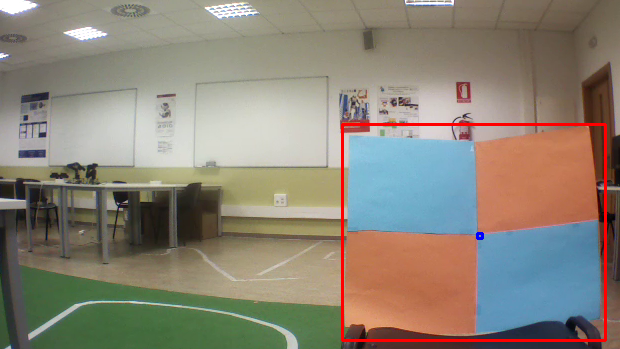
\includegraphics[width=7cm, height=3cm]{imgs/k_beacon21.png}}
  \subfloat[Suma de objetos]{
   \label{f:sumaobjetos}
    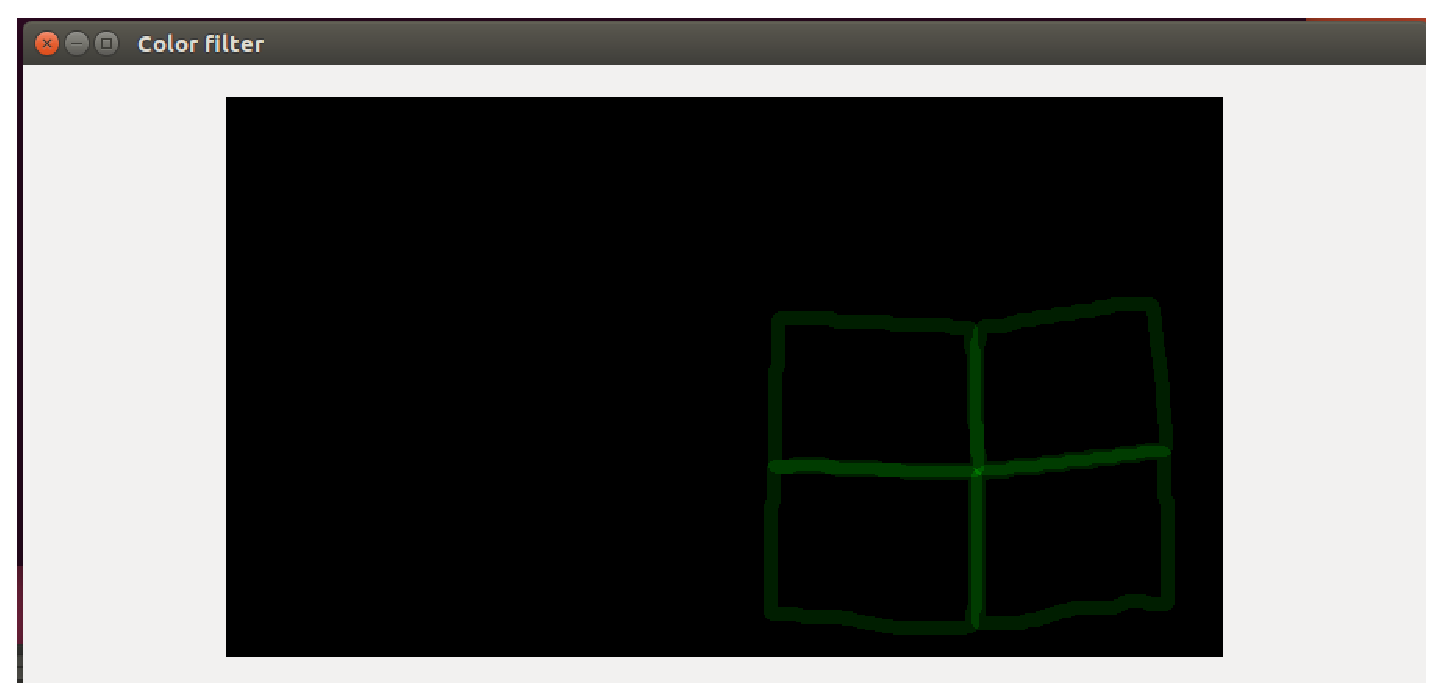
\includegraphics[width=7cm, height=3cm]{imgs/k_Beacon1.eps}} 
 \caption{Procesamiento de imagen de la baliza}
 \label{f:ColorFilterTotal}
\end{figure} 



\section{Control}
\label{sec.control}

\hspace{1 cm} En esta secci\'on se explica el control sobre el drone en funci\'on del momento del comportamiento en el que se encuentra y la imagen que se obtiene. Se puede dividir en tres partes:
despegue, b\'usqueda y aterrizaje. La figura \ref{fig:Esquema_control2} indica el esquema de control que sigue el algoritmo, los estados que est\'an en el mismo color, pertenecen a la parte de b\'usqueda, los otros dos, al despegue y aterrizaje:

\begin{figure}[H]
	\centering
		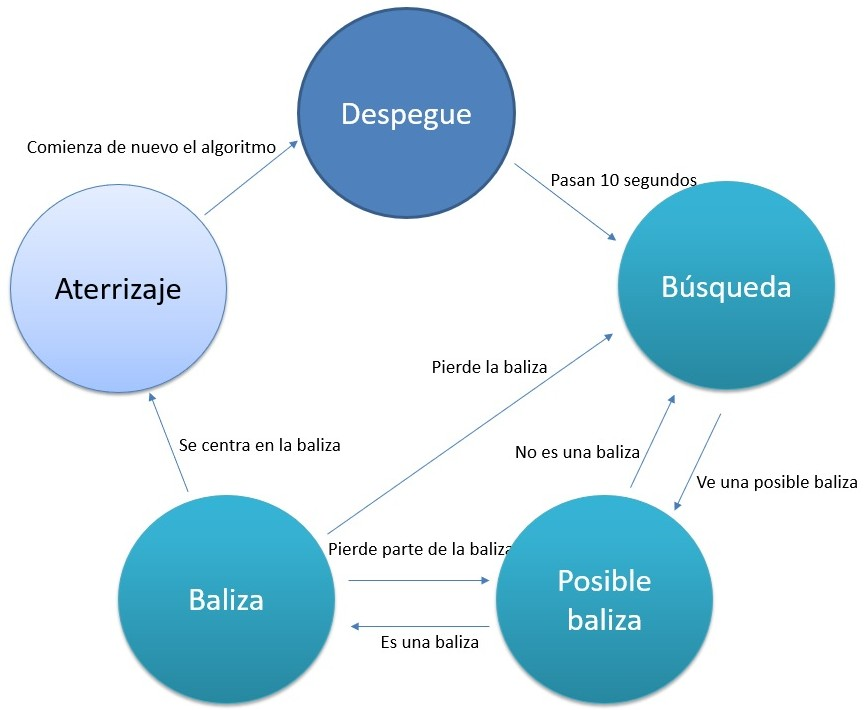
\includegraphics[width=0.6\textwidth]{imgs/NuevoAlgoritmo.jpg}
        \caption{Esquema de control del algoritmo.}
	\label{fig:Esquema_control2}
\end{figure}


\subsection{Despegue}

\hspace{1 cm} Esta fase est\'a controlada por tiempo. Son los primeros diez segundos del algoritmo, y en ellos el drone despega de forma controlada. Esta fase ser\'a "`Take off"' en el aut\'omata de estados de la figura \ref{fig:Diag_estados2}. Para ello se sit\'ua el drone sobre una baliza sobre la cual tiene que estabilizarse. De esta forma, al despegar detecta \'esta y trata de centrarse, evitando as\'i que se desv\'ie por factores externos y qued\'andose en la situaci\'on correcta. Debido a que el drone va a despegar sobre la baliza, el control en esta parte es un control proporcional, para evitar que tenga que hacer m\'ultiples operaciones, por tanto sea mas r\'apido el algoritmo, y suficiente para ser controlado.


\begin{figure}[ht]
	\centering
		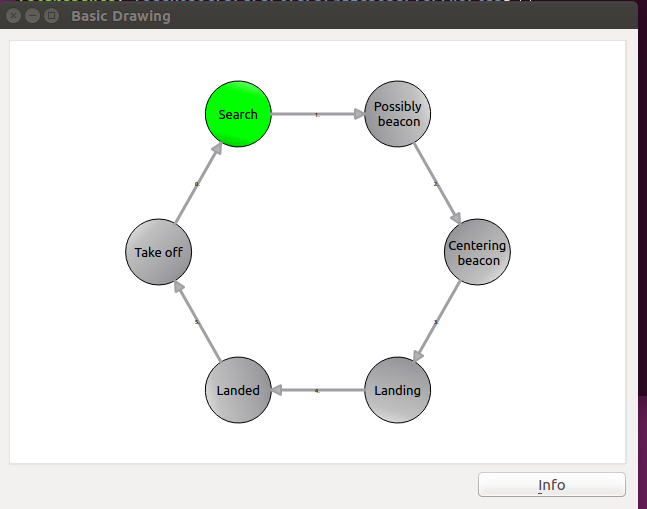
\includegraphics[width=0.7\textwidth]{imgs/states.png}
        \caption{Diagrama de estados utilizado para el algoritmo.}
	\label{fig:Diag_estados2}
\end{figure}


\subsection{B\'usqueda}
\hspace{1 cm} Esta fase empieza cuando finalicen los diez segundos de despegue. El drone comenzar\'a a navegar de forma aut\'onoma en b\'usqueda de una baliza sobre la cual aterrizar. Para ello sigue una navegaci\'on en espiral, estado "`Search"' de la figura \ref{fig:Diag_estados2}, de forma que ir\'a rastreando la zona ampliando su giro de forma continua, hasta que detecte una posible baliza. En el momento que la detecte, pasar\'a al estado "`Possibly beacon"' de la figura \ref{fig:Diag_estados2} e intentar\'a centrarse sobre ella. Si tras un n\'umero definido de iteraciones, no se detecta una b\'aliza, continuar\'a el algoritmo de b\'usqueda en el punto donde se hab\'ia quedado, aumentando con la amplitud de las espirales a la que se hab\'ia llegado. Pero en caso de detectarla pasar\'a al estado "`Centering beacon"' de la figura \ref{fig:Diag_estados2}, haciendo que coincida el centro de la baliza con el centro de la imagen de la c\'amara. Para realizar el movimiento de centrarse en la baliza se ha utilizado un control PD (proporcional y derivativo). Esto se debe a que s\'olo con el control proporcional, se produc\'ia una gran diferencia de velocidad y el drone cambiaba sus giros de forma muy brusca, lo que le llevaba a desestabilizarse y perder con facilidad la baliza. El algoritmo del control PD es de la siguiente forma:

\begin{itemize}
\item Por una parte, se tiene el control proporcional. Para \'este se obtiene el centro de la cruceta o del objeto de inter\'es. Se calcula la diferencia entre el centro de la imagen y el centro del objeto o la cruceta, obteniendo as\'i el error, y como resultados, para el eje x $\Delta_x$,  y para el eje y $\Delta_y$. Estos valores se multiplican por una constante que sirve para adaptar el resultado a la velocidad del drone. La f\'ormula de este control es la siguiente:  \[\Delta_x = centroimagen_x - centroobjeto_x\]   \[\Delta_y = centroimagen_y - centroobjeto_y\]  \[ P_x = \Delta_x * 0.01\]  \[P_y = \Delta_y * 0.01\]


\item Por otro lado, est\'a el control derivativo. Para este caso, al tratarse de iteraciones, se trabaja con las diferentes muestras de cada iteración. Se obtiene el error de la iteraci\'on actual y de la iteraci\'on anterior para ambos ejes, y se resta el error anterior al actual: \[\Delta_d_i_f_e_r_e_n_c_i_a_x =  \Delta_x [n] - \Delta_x [n-1] \] \[\Delta_d_i_f_e_r_e_n_c_i_a_y =  \Delta_y [n] - \Delta_y [n-1] \]  \[ D_x = \Delta_d_i_f_e_r_e_n_c_i_a_x * 0.003\]  \[D_y = \Delta_d_i_f_e_r_e_n_c_i_a_y * 0.003\]

\end{itemize}

\hspace{1 cm} Una vez se ha obtenido esto, se env\'ian las instrucciones de velocidad al drone, utilizando el comando:
\begin{lstlisting}[backgroundcolor=\color{yellow}]
vely = (y_img-positionY)                        
velx = (x_img-positionX)

Kp=0.01
vy_P = vely*Kp 
vx_P = velx*Kp

Kd = 0.003
vx_D = abs(xanterior-velx)*Kd
vy_D = abs(yanterior-vely)*Kd

Vy_tot = vy_P + vy_D
Vx_tot = vx_P + vy_D
self.cmdvel.sendCMDVel(Vy_tot,Vx_tot,0,0,0,0) 

xanterior = velx
yanterior = vely

if(abs(Vx_tot-xanteriorTot)>0.3):
   if(Vx_tot<xanteriorTot):
      Vx_tot = xanteriorTot-0.3
   else:
      Vx_tot = xanteriorTot+0.3                                 

if(abs(Vy_tot-yanteriorTot)>0.3):
   if(Vy_tot<yanteriorTot):
      Vy_tot = yanteriorTot-0.3
   else:
      Vy_tot = yanteriorTot+0.3                                 
yanteriorTot = vytot
xanteriorTot = vxtot

self.cmdvel.sendCMDVel(Vy_tot,Vx_tot,0,0,0,0) 
\end{lstlisting}
	

 %$\\ Calculo \Delta_x : \[\Delta_x = centroimagen_x - centroobjeto_x\] \\ Calculo \Delta_x : \[\Delta_y = centroimagen_y - centroobjeto_y\] \\ Calculo del control proporcional P_x : \[ P_x = \Delta_x * 0.01\] \\ Calculo del control proporcional P_y : \[P_y = \Delta_y * 0.01\] 




%\hspace{1 cm} Esta fase comenzar\'a cuando finalicen los diez segundos de despegue. El drone comenzar\'a a navegar de forma aut\'onoma en b\'usqueda de una baliza sobre la cual aterrizar. Para ello comenzar\'a un algoritmo en espiral, estado "`Search"', de forma que ir\'a rastreando la zona ampliando su giro de forma continua, hasta que detecte una posible baliza. En el momento que la detecte, pasar\'a al estado "`Possibly beacon"' e intentar\'a centrarse sobre ella. En caso de no tratarse de la baliza, continuar\'a con el algoritmo de b\'usqueda, pero en caso de serlo pasar\'a al estado "`Centering beacon"', haciendo que coincida el centro de la baliza con el centro de la imagen de la c\'amara. Para realizar el movimiento de centrarse en la baliza se ha utilizado un control PID (progresivo, integral y derivativo). Esto se debe a que s\'olo con el control progresivo, se produc\'ia una gran diferencia de velocidad y el drone cambiaba sus giros de forma muy brusca, lo que le llevaba a desestabilizarse y perder con facilidad la baliza.  Este control se basa en derivar el error con respecto al tiempo y multiplicarlo por una constante. Dado que nuestro algoritmo ejecuta una vez cada cierto tiempo y no esta continuamente pasando por este punto, podemos considerar que se trata de un sistema en tiempo discreto, y por tanto en lugar de trabajar con derivadas trabajaremos con sumatorios. De esta forma, para añadir un control derivativo se realiza una operaci\'on que depende de la velocidad anterior y la que tenemos ahora: \[v_{derivativa} =1-(v_{anterior}-v_{nueva})/50 \] 

%\hspace{1cm}Para evitar que el valor sea 0 y al multiplicarlo por el valor progresivo se quede en el sitio, en caso de ser un valor menor a 0.1 se iguala a \'este. Este resultado lo multiplicamos a la velocidad final, y lo que conseguimos es que si el valor entre dos velocidades continuas es muy alto, \'este se aten\'ue de forma que el drone no cambie mucho y vaya oscilando, sino que lleve una velocidad m\'as continua a la hora de acelerar o frenar.  

El siguiente fragmento de c\'odigo consigue que el drone se mueva realizando espirales: \\

\begin{lstlisting}[backgroundcolor=\color{yellow}]
self.cmdvel.sendCMDVel(1.8+wSearch,0,0,0,0,1.5 - wSearch)
numVuelta=numVuelta+1
if(numVuelta==100):
    timerW=timerW+(timerW/8)
    numVuelta=0
    if(wSearch<1):
        wSearch=wSearch+0.2
\end{lstlisting}

\hspace{1 cm} El esquema de este control cuando el drone est\'a en el estado de b\'usqueda es el siguiente:
\begin{figure}[ht]
	\centering
		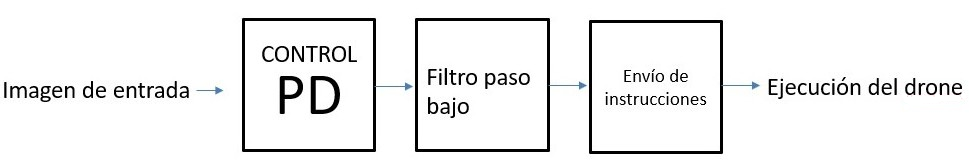
\includegraphics[width=1\textwidth]{imgs/esquemapd2.png}
        \caption{Esquema de control durante el algoritmo de b\'usqueda}
	\label{fig:Esquema_control}
\end{figure}


\subsection{Aterrizaje}

\hspace{1 cm} Esta fase es un aterrizaje controlado. Una vez el drone se ha centrado sobre la baliza comienza a descender de forma constante , cambiando el estado a "`Landing"'. Cuando \'area es menor a cierto umbral (en p\'ixeles), en \'este caso 19272135.0, se manda la instrucci\'on de parar motores. En ese momento el drone desciende hasta posarse en el suelo, entonces para los motores y el estado cambia a "`Landed"'. La raz\'on de ir descendiendo poco a poco hasta detectar determinado \'area, es por si la baliza est\'a lejos del drone, puede interferir alg\'un objeto moment\'aneamente o darse alg\'un factor externo que altere la posici\'on del drone respecto de la baliza, y al enviar la instrucci\'on de parar motores se perder\'ia este control. El umbral elegido es porque en ese momento la baliza ocupa pr\'acticamente por completo la imagen, y si se le indicara al drone que siguiera descendiendo las corrientes que se producir\'ian con el suelo podr\'ian afectarle y desviar su trayectoria, pudiendo perder la referencia.


%\hspace{1 cm} Una vez finalizada la descripci\'on del algoritmo completo, un esquema del control completo es el siguiente:



%Esta fase es un aterrizaje controlado, en el cual, una vez que el drone se ha centrado sobre la baliza comienza a descender, cambiando su estado a "`Landing"', y una vez el \'area de la baliza es suficiente, como para detectar que el drone est\'a muy pr\'oximo a ella, se env\'ia la instrucci\'on land, aterrizando de \'esta forma el drone, siendo aqu\'i su estado "`Landed"'. El hecho de enviarse la orden de aterrizar cuando se est\'a a una distancia cercana a la baliza es porque esta instrucci\'on es a ciegas, una vez que se env\'ia el drone solo se encarga de descender hasta que nota que est\'a sobre un lugar sobre el cual posarse. Por lo tanto si se env\'ia esta orden a una distancia lejana, el drone puede perder la referencia y aterrizar en otro sitio. 



\section{Arquitectura software de la implementaci\'on}

\hspace{1 cm} El programa tiene que funcionar con fluidez, permitiendo enviar y recibir datos a la vez que se visualizan los datos que ya se tienen. Para ello, la aplicaci\'on PreciseLanding tiene una estructura que sigue el siguiente esquema:
%ENVIAR DATOS Y RECIBIR ORDENES

\hspace{1 cm} Primero est\'a el programa principal precise\_landing.py. \'Este es el encargado de crear la m\'aquina de estados, decir el n\'umero de estados que va a tener y las posibles transiciones entre unos y otros. Tambi\'en se conecta con los sensores y actuadores a trav\'es de las interfaces ICE creando los manejadores respectivos (c\'amara, datos de navegaci\'on, datos de posici\'on, comandos de velocidad y comandos extra para despegar y aterrizar) para pas\'arselos como par\'ametro a \'este. Una vez se tenga todo definido, se pasa a la creaci\'on de los distintos hilos.

\hspace{1 cm} Por un lado se crea el interfaz gr\'afica y la ventana en la que se muestra el diagrama de estados. Se hace que \'este se ejecute en un hilo y se le manda comenzar.

\hspace{1cm} Para visualizar el diagrama de estados, se añadieron dos paquetes del GUI, uno que permit\'ia abrir otra ventana y otro que permit\'ia añadir estados y transiciones entre ellos. Para marcarlo, siendo el numero que aparece el numero del estado que queremos marcar, val\'ia con la siguiente linea de c\'odigo:

\begin{lstlisting}[backgroundcolor=\color{yellow}]
self.machine.setStateActive(2, True)
\end{lstlisting}
	
\hspace{1cm}La imagen del diagrama que ver\'iamos durante la ejecuci\'on se encuentra en \ref{fig:Diag_estados2}. La imagen cuando se abre la aplicaci\'on, es la que se encuentra en \ref{f:pl2}

\hspace{1 cm} Por otro lado, se crea la ventana gr\'afica de control, que permite el control del drone y muestra la informaci\'on de sus sensores. A \'este se le pasan como datos los distintos manejadores anteriormente definidos para que pueda utilizarlas, como son la c\'amara para visualizar las imagenes o el \textit{cmdvel} para enviar las ordenes de velocidad. Esta ventana tambi\'en tiene los botones de "Play" y "Stop", los cuales permiten que ejecute el algoritmo creado o que pare su ejecuci\'on. Esta interfaz corresponde con la imagen \ref{f:pl1}.

\hspace{1 cm} Para finalizar se llama a la funci\'on que ejecutar\'a el algoritmo principal. A esta funci\'on se le pasan como parametros todo lo hasta ahora creado, para que as\'i pueda acceder a los datos de la c\'amara, los distintos sensores y el diagrama de estados. Esta funci\'on permitir\'a obtener los datos deseados de los sensores, enviar instrucciones a los motores y al diagrama de estados. Este algoritmo, adem\'as de tener la funci\'on principal y las creadas para el funcionamiento de este, tiene cuatro funciones esenciales para su funcionamiento. Por un lado est\'an las funciones de "play" y "stop" (asociadas a los botones respectivos de la ventana gr\'afica de control), las cuales mandan el evento de iniciar (en caso de la funci\'on Play), de parar (en caso de la funci\'on Stop), que se ejecutaran principalmente cuando se pulsen los botones del interfaz de control. Por otro lado est\'a la funci\'on "kill"", que se encarga de matar el proceso. Por \'ultimo est\'a la funci\'on "run", que es la encargada de llamar de forma continua al algoritmo a ejecutar mientras no se mate a la aplicaci\'on. Esta funci\'on, mientras se haya mandado la instrucci\'on de iniciar y no la de parar, se encontrar\'a en un bucle continuo obteniendo a final de cada iteraci\'on el tiempo que ha tardado en ejecutarse, en caso de no llegar a un m\'inimo de tiempo, la funci\'on parara la cantidad de tiempo necesaria para llegar a ese m\'inimo, y entonces dejar\'a continuar con la ejecuci\'on. De esta forma, la velocidad de iteraciones no s\'olo depender\'a del algoritmo y las funciones en si, sino que en caso de tardar muy poco tendr\'a determinados tiempos de espera.



\begin{figure}[H]
 \centering
  \subfloat[Precise Landing]{
   \label{f:pl1}
    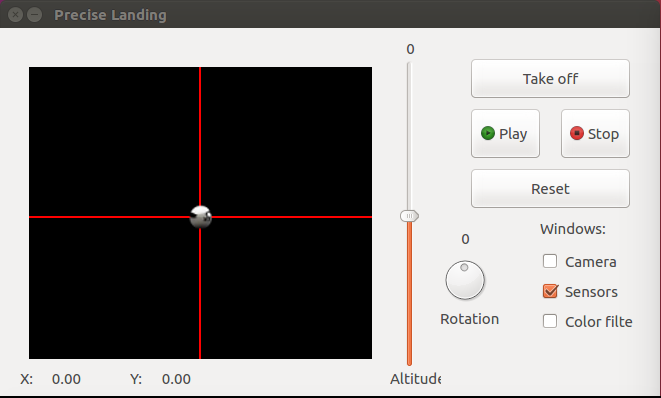
\includegraphics[width=7cm, height=3.7cm]{imgs/PreciseLanding1.png}}
  \subfloat[Diagrama de Estados]{
   \label{f:pl2}
    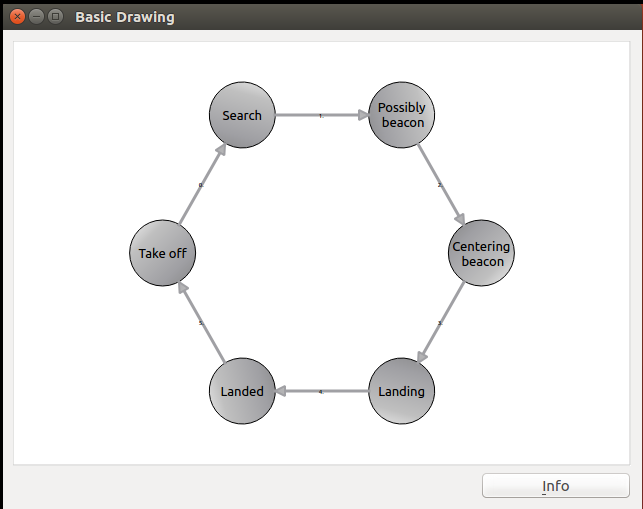
\includegraphics[width=7cm, height=3.7cm]{imgs/PreciseLanding2.png}} 
 \caption{Interfaces que se abren al iniciar la aplicaci\'on.}
 \label{f:PreciseLanging}
\end{figure}













